%%%%(c)
%%%%(c)  This file is a portion of the source for the textbook
%%%%(c)
%%%%(c)    Abstract Algebra: Theory and Applications
%%%%(c)    Copyright 1997 by Thomas W. Judson
%%%%(c)
%%%%(c)  See the file COPYING.txt for copying conditions
%%%%(c)
%%%%(c)
\chap{Group Actions}{actions}

Group actions generalize group multiplication.  If $G$ is a group and $X$ is an arbitrary set, a group action of an element $g \in G$ and $x \in X$ is a product, $gx$,  living in $X$.  Many problems in algebra may best be attacked via group actions.  For example, the proofs of the Sylow theorems and of Burnside's Counting Theorem are most easily understood when they are formulated in terms of group actions. 


\section{Groups Acting on Sets}

Let $X$ be a set and $G$ be a group.  A  {\bfi (left) action\/}\index{Group!action} of $G$ on $X$ is a map $G \times X \rightarrow X$ given by $(g,x) \mapsto gx$, where 
\begin{enumerate}
 
\item 
$ex = x$ for all $x \in X$;
 
\item 
$(g_1 g_2)x = g_1(g_2 x)$ for all $x \in X$ and all $g_1, g_2 \in G$. 
 
\end{enumerate}
Under these considerations $X$ is called a {\bfi $G$-set}\index{$G$-set}.  Notice that we are not requiring $X$ to be related to $G$ in any way.  It is true that every group $G$ acts on every set $X$ by the trivial action $(g,x) \mapsto x$; however, group actions are more interesting if the set $X$ is somehow related to the group $G$. 

\begin{example}{GL2_action}
Let $G = GL_2( {\mathbb R} )$ and $X = {\mathbb R}^2$. Then $G$ acts on $X$ by left multiplication.  If $v \in {\mathbb R}^2$ and $I$ is the identity matrix, then $Iv = v$.  If $A$ and $B$ are $2 \times 2$ invertible matrices, then $(AB)v = A(Bv)$ since matrix multiplication is
associative. 
\end{example}

\begin{example}{D4_action}
Let $G = D_4$ be the symmetry group of a square.  If $X = \{ 1, 2, 3, 4 \}$ is the set of vertices of the square, then we can consider $D_4$
to consist of the following permutations: 
\[
\{ (1), (13), (24), (1432), (1234), (12)(34), (14)(23), (13)(24) \}.
\]
The elements of $D_4$ act on $X$ as functions.  The permutation $(13)(24)$ acts on vertex 1 by sending it to vertex 3, on vertex 2 by
sending it to vertex 4, and so on.  It is easy to see that the  axioms of a group action are satisfied.
\mbox{\hspace{1in}}
\end{example}



In general, if $X$ is any set and $G$ is a subgroup of $S_X$, the
group of all permutations acting on $X$, then $X$ is a $G$-set under
the group action 
\[
(\sigma, x) \mapsto \sigma(x)
\]
for $\sigma \in G$ and $x \in X$.
 
 
\begin{example}{left_action}
If we let $X = G$, then every group $G$ acts on itself by the left
regular representation; that is, $(g,x) \mapsto \lambda_g(x) = gx$, 
where  $\lambda_g$ is left multiplication:
\begin{gather*}
e \cdot x = \lambda_e x = ex = x \\
(gh) \cdot x = \lambda_{gh}x = \lambda_g \lambda_h x =
\lambda_g(hx) = g \cdot ( h \cdot x).
\end{gather*}
If $H$ is a subgroup of $G$, then $G$ is an $H$-set under left
multiplication by elements of $H$. 
\end{example}
 
 
\begin{example}{conj_action}
Let $G$ be a group and suppose that $X=G$. If $H$ is a subgroup of
$G$, then $G$ is an $H$-set under {\bfi
conjugation}\index{Conjugation}; that is, we can define an action of
$H$ on $G$, 
\[
H \times G \rightarrow G,
\]
via
\[
(h,g) \mapsto hgh^{-1}
\]
for $h \in H$ and $g \in G$.  Clearly, the first axiom for a group
action holds.  Observing that 
\begin{align*}
(h_1 h_2, g) 
& = h_1 h_2 g (h_1 h_2 )^{-1} \\
& = h_1( h_2 g h_2^{-1}) h_1^{-1} \\
& =  (h_1, (h_2, g) ),
\end{align*}
we see that the second condition is also satisfied.
\end{example}
 
 
\begin{example}{left_coset_action}
Let $H$ be a subgroup of $G$ and ${\mathcal L}_H$ the set of left cosets
of $H$.  The set ${\mathcal L}_H$ is a $G$-set under the action
\[
(g, xH) \mapsto gxH.
\]
Again, it is easy to see that the first axiom is true. Since $(g g')xH
= g( g'x H)$, the second axiom is  also true.
\end{example}
 
 
 
If $G$ acts on a set $X$ and $x, y \in X$, then $x$ is said to be
{\bfi  $G$-equivalent\/}\index{$G$-equivalent} to $y$ if there exists a
$g \in G$ such that $gx =y$. We  write $x \sim_G y$ or $x \sim y$ if
two elements are $G$-equivalent. 
 
 
\begin{proposition}
Let  $X$ be a $G$-set. Then $G$-equivalence is an equivalence relation
on $X$. 
\end{proposition}
 
 
\begin{proof}
The relation $\sim$ is reflexive since $ex = x$. Suppose that $x \sim
y$ for $x, y \in X$. Then there exists a $g$ such that $gx = y$. In
this case $g^{-1}y=x$; hence, $y \sim x$. To show that the relation is
transitive, suppose that $x \sim y$ and $y \sim z$. Then there must
exist group elements $g$ and $h$ such that $gx = y$ and $hy= z$. So $z
= hy = (hg)x$, and  $x$ is equivalent to $z$.
\end{proof}
 
 
\medskip
 
 
If $X$ is a $G$-set, then each partition of $X$ associated with
$G$-equivalence is called an {\bfi orbit\/}\index{Orbit} of $X$ under
$G$.  We will denote the orbit that contains an element $x$  of $X$ by
${\mathcal O}_x$\label{noteorbit}. 
 
 
\begin{example}{permute_action}
Let $G$ be the permutation group defined by
\[
G =\{(1), (1 2
3), (1 3 2), (4 5), (1 2 3)(4 5), (1 3 2)(4 5) \}
\]
and $X = \{ 1, 2, 3, 4, 5\}$. Then $X$ is a $G$-set. The orbits are
${\mathcal O}_1 = {\mathcal O}_2 = {\mathcal O}_3 =\{1, 2, 3\}$ and $ {\mathcal O}_4=
{\mathcal O}_5 = \{4, 5\}$. 
\end{example}
 
 

 
 
Now suppose that $G$ is a group acting on a set $X$ and let $g$ be
an element of $G$. The {\bfi fixed point set\/}\index{Fixed point
set} of $g$ in $X$, denoted by $X_g$\label{notefixed}, is the set of 
all $x \in X$ such
that $gx = x$.  We can also study the group elements $g$ that fix a
given $x \in X$. This set is more than a subset of  $G$, it is a
subgroup.  This subgroup is called the {\bfi stabilizer 
subgroup\/}\index{Subgroup!stabilizer} or {\bfi isotropy 
subgroup\/}\index{Subgroup!isotropy} of $x$. We will denote the 
stabilizer subgroup of $x$ by $G_x$\label{noteisotropy}. 
 
 
\medskip
 
 
\noindent {\bf Remark.}  
It is important to remember that $X_g \subset X$ and $G_x \subset G$. 
 
 
\begin{example}{stabilizer_action}
Let $X = \{1, 2, 3, 4, 5, 6\}$ and suppose that $G$ is the permutation
group given by the permutations 
\[
\{
(1), (1 2)(3 4 5 6), (3 5)(4 6), (1 2)( 3 6 5 4)
\}.
\]
Then the fixed point sets  of $X$ under the action of $G$ are
\begin{gather*}
X_{(1)}  =  X, \\
X_{(3 5)(4 6)}  =  \{1,2\}, \\
X_{(1 2)(3 4 5 6)}  = X_{(1 2)(3 6 5 4)}  =  \emptyset,
\end{gather*}
and the stabilizer subgroups are
\begin{gather*}
G_1 =  G_2  =  \{(1), (3 5)(4 6) \}, \\
G_3  = G_4  = G_5  = G_6 =  \{(1)\}.
\end{gather*}
It is easily  seen that  $G_x$ is a subgroup of $G$ for each $x \in
X$. 
\end{example}
 
 
\begin{proposition}
Let $G$ be a  group acting on a set $X$ and $x \in X$. The stabilizer
group, $G_x$, of $x$ is a subgroup of $G$. 
\end{proposition}
 
 
\begin{proof}
Clearly,  $e \in G_x$ since the identity fixes every element in the
set $X$. Let $g, h \in G_x$. Then $gx = x$ and $hx = x$. So $(gh)x =
g(hx) = gx = x$; hence, the product of two elements in $G_x$ is also
in $G_x$. Finally, if $g \in G_x$, then $x = ex = (g^{-1}g)x =
(g^{-1})gx = g^{-1} x$. So $g^{-1}$ is in $G_x$. 
\end{proof}
 
 
\medskip
 
 
We will denote the number of elements in the fixed point set of an
element $g \in G$ by $|X_g|$ and denote the number of elements in the
orbit of $x \in X$ by $|{\mathcal O}_x|$. The next theorem
demonstrates the relationship between orbits of an element $x \in X$
and the left cosets of $G_x$ in $G$.

%typo corrected.  Suggested by L. Franklin.
%TWJ - 12/19/2011
 
 
\begin{theorem}\label{orbit_theorem}
Let $G$ be a finite group and $X$ a finite $G$-set. If $x \in X$,
then $|{\mathcal O}_x| = [G:G_x]$. 
\end{theorem}
 
 
\begin{proof}
We know that  $|G|/|G_x|$ is the number of left cosets of $G_x$ in $G$
by Lagrange's Theorem (Theorem~\ref{LagrangeTheorem}). We will define a bijective  map $\phi$
between the orbit ${\mathcal O}_x$ of $X$ and the set of left cosets 
${\mathcal L}_{G_x}$ of $G_x$ in $G$. Let $y \in {\mathcal O}_x$. Then there 
exists a $g$ in $G$ such that $g x = y$. Define $\phi$ by $\phi( y ) 
= g G_x$. First we must show that this map is well-defined and does 
not depend on our selection of $g$. Suppose that $h$ is another 
element in $G$ such that $hx = y$. Then $g x = h x$ or $x= g^{-1} h x$; 
hence, $g^{-1}h$ is in the stabilizer subgroup of $x$. Therefore, 
$h \in g G_x$ or $g G_x = h G_x$.  Thus, $y$ gets mapped to the same 
coset regardless of the choice of the representative from that coset.
 
 
To show that $\phi$ is one-to-one, assume that $\phi(x_1) =
\phi(x_2)$. Then there exist $g_1, g_2 \in G$ such that $x_1 = g_1 x$
and $x_2 = g_2 x$. Since there exists a $g \in G_x$ such that $g_2=g_1
g$, 
\[
x_2 = g_2 x = g_1 g x = g_1 x = x_1;
\]
consequently, the map $\phi$ is  one-to-one. Finally, we must show
that the map $\phi$ is onto. Let $g G_x$ be a left coset. If $g x =
y$, then $\phi(y) = g G_x$. 
\end{proof}
 
 
 
 
\section{The Class Equation}
 
 
 
Let $X$ be a finite $G$-set and $X_G$\label{noteXG} be the set of fixed 
points in $X$; that is, 
\[
X_G = \{ x \in X : gx = x \mbox{ for all $g \in G$} \}.
\]
Since the orbits of the action partition $X$,
\[
|X| = |X_G| + \sum_{i = k}^n |{\mathcal O}_{x_i}|,
\]
where $x_k, \ldots, x_n$ are representatives from the distinct
nontrivial orbits of $X$. 
 
 
Now consider the special case in which $G$ acts on itself by conjugation,
$(g,x) \mapsto gxg^{-1}$. The {\bfi center\/}\index{Group!center of} of
$G$, 
\[
Z(G) = \{x : xg = gx \mbox{ for all $g \in G$} \},
\]
is the set of points that are fixed by conjugation. The nontrivial
orbits of the action are called the {\bfi conjugacy
classes\/}\index{Conjugacy classes} of $G$. If $x_1, \ldots, x_k$ are
representatives from each of the nontrivial conjugacy classes of $G$
and $|{\mathcal O}_{x_1}| = n_1, \ldots, |{\mathcal O}_{x_k}| = n_k$, then 
\[
|G| = |Z(G)| + n_1 + \cdots + n_k.
\]
The stabilizer subgroups of each of the $x_i$'s, $C(x_i) = \{ g \in G
: g x_i = x_i g \}$, are called the {\bfi centralizer
subgroups\/}\index{Subgroup!centralizer}\index{Centralizer!of a
subgroup} of the $x_i$'s. From Theorem~\ref{orbit_theorem}, we obtain the {\bfi class
equation\/}\index{Class equation}: 
\[
|G| = |Z(G)| + [G: C(x_1) ] + \cdots + [ G: C(x_k)].
\]
One of the consequences of the class equation is that the order of
each conjugacy class must divide the order of $G$.
%Reference repaired. TWJ 12/19/2011
%Typo corrected. Suggested by A. Vance. TWJ 11/13/2011
 
\begin{example}{conjugacy_class_S3}
It is easy to check that  the conjugacy classes in $S_3$ are the
following: 
\[
\{ (1) \},  \quad \{ (123), (132) \}, \quad \{(12), (13), (23) \}.
\]
The class equation is $6 = 1+2+3$.
\end{example}
 
 
\begin{example}{conjugacy_class_D4} 
The center of $D_4$ is $\{ (1), (13)(24) \}$, and the conjugacy classes are
\[
\{ (13), (24) \}, \quad
\{ (1432), (1234) \}, \quad
\{ (12)(34), (14)(23) \}.
\]
Thus, the class equation for $D_4$ is $8 = 2 + 2 + 2 + 2$.
\end{example}
%%Example corrected.  There are 5 classes. TWJ 9/7/2010
%%Example clarified.  Suggested by B. Whetter.  TWJ 11/17/2012
 
 
\begin{example}{Conjugacy_Class_Sn}
For $S_n$ it takes a bit of work to find the conjugacy classes.  We
begin with cycles.  Suppose that $\sigma = ( a_1, \ldots, a_k)$ is a
cycle and let $\tau \in S_n$. By Theorem~\ref{cosets:cycle_length_theorem},
\[
\tau \sigma \tau^{-1} = ( \tau( a_1), \ldots, \tau(a_k)).
\]
Consequently, any two cycles of the same length are conjugate. Now let
$\sigma = \sigma_1 \sigma_2 \cdots \sigma_r$ be a cycle decomposition,
where the length of each cycle $\sigma_i$ is $r_i$. Then $\sigma$ is
conjugate to every other $\tau \in S_n$ whose cycle decomposition has
the same lengths. 
 
 
The number of conjugate classes in $S_n$ is the number of ways in
which $n$ can be partitioned into sums of positive integers. For
example, we can partition the integer 3 into the following three sums: 
\begin{align*}
3 & =  1 + 1 + 1 \\
3 & =  1 + 2 \\
3 & =  3;
\end{align*}
therefore, there are three conjugacy classes. The problem of finding
the number of such partitions for any positive integer $n$ is what
computer scientists call {\bfi NP-complete}.  This effectively means
that the problem cannot be solved for a large $n$ because the
computations would be too time-consuming for even the largest computer. 
\end{example}
 
 

 
 
\begin{theorem}\label{pn_theorem}
Let $G$ be a group of order $p^n$ where $p$ is prime. Then $G$ has a
nontrivial center. 
\end{theorem}
 
 
\begin{proof}
We apply the class equation
\[
|G| = |Z(G)|  + n_1 + \cdots + n_k.
\]
Since each $n_i>1$ and $n_i \mid |G|$, $p$  must divide each $n_i$.
Also, $p \mid |G|$; hence, $p$ must divide $|Z(G)|$. Since the
identity is always in the center of $G$, $|Z(G)| \geq 1$. Therefore,
$|Z(G)|  \geq p$ and there exists some $g \in Z(G)$ such that $g \neq
1$. 
\mbox{\hspace*{1in}} 
\end{proof}
%Typo fixed.  Suggested by A. Vance.  TWJ 11/17/2012
 
 
\begin{corollary}\label{actions:p2abelian}
Let $G$ be a group of order $p^2$ where $p$ is prime. Then $G$ is
abelian. 
\end{corollary}
 
 
\begin{proof}
By Theorem~\ref{pn_theorem}, $|Z(G)| = p$ or $p^2$.  If $|Z(G)| = p^2$, then
we are done.  Suppose that $|Z(G)| = p$. Then $Z(G)$ and $G / Z(G)$
both have order $p$ and must both be cyclic groups.  Choosing  a
generator $aZ(G)$ for $G / Z(G)$, we can write any element $gZ(G)$ in
the quotient group as $a^m Z(G)$ for some integer $m$; hence, $g = a^m
x$ for some $x$ in the center of $G$.  Similarly, if $hZ(G) \in G /
Z(G)$, there exists a $y$ in $Z(G)$ such that $h = a^n y$ for some
integer $n$.  Since $x$ and $y$ are in the center of $G$, they commute
with all other elements of $G$; therefore, 
\[
gh  =  a^m x a^n y =  a^{m+n} x y = a^n y a^m x = hg,
\]
and $G$ must be abelian.
\end{proof}
 
 
 
\section{Burnside's Counting Theorem}
 
 
 
Suppose that we are to color the vertices of a square with two
different colors, say black and white.  We might suspect that there
would be $2^4=16$ different colorings. However, some of these
colorings are equivalent.  If we color the first vertex black and the
remaining vertices white, it is the same as coloring the second vertex
black and the remaining ones white since we could obtain the second
coloring simply by rotating the square $90^\circ$
(Figure~\ref{colorings}). 
 
\begin{figure}[htb]

\begin{center}
\tikzpreface{actions_colorings_square}
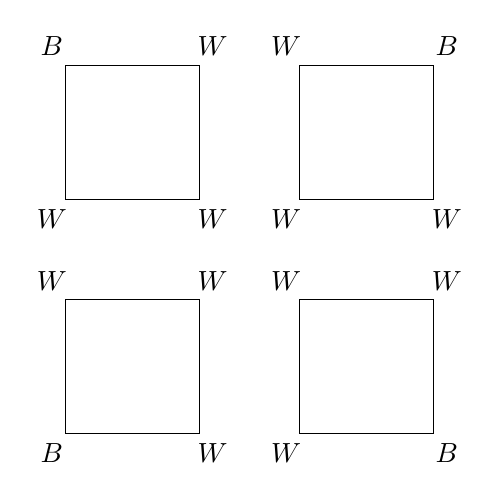
\begin{tikzpicture}[scale=0.85] %%Replaced figure with tikz figure - TWJ 6/28/2010

\draw (0,0) rectangle (2,2);
\node at (-0.2,0) [below] {$B$};
\node at (2.2,0) [below] {$W$};
\node at (-0.2,2) [above] {$W$};
\node at (2.2,2) [above] {$W$};

\draw (3.5,0) rectangle (5.5,2);
\node at (3.3,0) [below] {$W$};
\node at (5.7,0) [below] {$B$};
\node at (3.3,2) [above] {$W$};
\node at (5.7,2) [above] {$W$};

\draw (0,3.5) rectangle (2,5.5);
\node at (-0.2,3.5) [below] {$W$};
\node at (2.2,3.5) [below] {$W$};
\node at (-0.2,5.5) [above] {$B$};
\node at (2.2,5.5) [above] {$W$};


\draw (3.5,3.5) rectangle (5.5,5.5);
\node at (3.3,3.5) [below] {$W$};
\node at (5.7,3.5) [below] {$W$};
\node at (3.3,5.5) [above] {$W$};
\node at (5.7,5.5) [above] {$B$};

\end{tikzpicture}
\end{center}
\caption{Equivalent colorings of square}
\label{colorings}
\end{figure}
 
 
Burnside's Counting Theorem offers a method of computing the number of
distinguishable ways in which something can be done. In addition to
its geometric applications, the theorem has interesting applications
to areas in switching theory and chemistry. The proof of Burnside's
Counting Theorem depends on the following lemma.
 
 
\begin{lemma}\label{Gset_lemma}
Let $X$ be a $G$-set and suppose that $x \sim y$. Then $G_x$ is
isomorphic to $G_y$.  In particular, $|G_x| = |G_y|$. 
\end{lemma}
 
 
 %% Notation error pointed out by S. Engle corrected.
 %% TWJ 11/20/2011

\begin{proof}
Let $G$ act on $X$ by $(g,x) \mapsto g \cdot x$. Since $x \sim y$,
there exists a $g \in G$ such that $g \cdot x=y$. Let $a \in G_x$.
Since 
\[
gag^{-1} \cdot y = ga \cdot g^{-1}y = ga \cdot x = g \cdot
x = y,
\]
we can define a map $\phi: G_x \rightarrow G_y$ by $\phi(a) =
gag^{-1}$. The map $\phi$ is a homomorphism since 
\[
\phi(ab) = gabg^{-1} = gag^{-1} gbg^{-1} = \phi(a) \phi(b).
\]
Suppose that $\phi(a) = \phi(b)$. Then $gag^{-1}= gbg^{-1}$ or $a=b$;
hence, the map is injective.  To show that $\phi$ is onto, let $b$ be
in $G_y$; then $g^{-1}bg$ is in $G_x$ since
\[
g^{-1}bg \cdot x = g^{-1}b \cdot gx = g^{-1}b \cdot y = g^{-1} \cdot y
= x; 
\]
and $\phi(g^{-1}bg ) = b$.
\end{proof}
 
 
\begin{theorem}[Burnside]\index{Burnside's Counting Theorem}
Let $G$ be a  finite group acting on a set $X$ and let $k$ denote the
number of orbits of $X$. Then
\[
k = \frac{1}{|G|} \sum_{g \in G} |X_g|.
\]
\end{theorem}
 
 
\begin{proof}
We look at all the fixed points $x$ of all the elements in $g \in G$;
that is, we look at all $g$'s and all $x$'s such that $gx =x$.
If viewed in terms of fixed point sets, the number of all $g$'s fixing
$x$'s is 
\[
\sum_{g \in G} |X_g|.
\]
However, if viewed in terms of the stabilizer subgroups, this number
is 
\[
\sum_{x \in X} |G_x|;
\]
hence, $\sum_{g \in G} |X_g| = \sum_{x \in X} |G_x|$. By Lemma~\ref{Gset_lemma}, 
\[
\sum_{y \in {\mathcal O}_x} |G_y|  =  | {\mathcal O}_x| \cdot |G_x|.
\]
By Theorem~\ref{orbit_theorem} and Lagrange's Theorem, this expression is equal 
to $|G|$. Summing over all of the $k$ distinct orbits, we conclude that
\[
\sum_{g \in G} |X_g| = \sum_{x \in X} |G_x| = k \cdot |G|.
\]
\end{proof}
 
 
\begin{example}{Burnside_example}
Let $X = \{1, 2, 3, 4, 5 \}$ and suppose that $G$ is the permutation
group $G= \{(1), (1 3), (1 3)(2 5), (2 5) \}$. The orbits of $X$ are
$\{1, 3\}$, $\{2, 5\}$, and $\{4\}$. The fixed point sets are 
\begin{align*}
X_{(1)} & =  X \\
X_{(1 3)} & =  \{2, 4, 5 \} \\
X_{(1 3)(2 5)} & =  \{4\} \\
X_{(2 5)} & =  \{1, 3, 4 \} .
\end{align*}
Burnside's Theorem says that
\[
k = \frac{1}{|G|} \sum_{g \in G} |X_g| = \frac{1}{4}(5+
3+1+3) = 3.
\]
\end{example}
 
 
 
\subsection*{A Geometric Example}
 
 
 
Before we apply Burnside's Theorem to switching-theory problems, let
us examine the number of ways in which the vertices of a square can be
colored black or white. Notice that we can sometimes obtain equivalent
colorings by simply applying a rigid motion to the square. For
instance, as we have pointed out, if we color one of the vertices
black and the remaining three white, it does not matter which vertex
was colored black since a rotation will give an equivalent coloring.  
 
 
The  symmetry group of a square, $D_4$, is given by the following
permutations: 
\[
\begin{array}{cccc}
(1)    & (13)     & (24)     & (1432) \\
(1234) & (12)(34) & (14)(23) & (13)(24)
\end{array}
\]
The group $G$ acts on the set of vertices $\{ 1, 2, 3, 4\}$ in the
usual manner. We can describe the different colorings by mappings from
$X$ into $Y = \{ B, W \}$ where $B$ and $W$ represent the colors black
and white, respectively. Each map $f : X \rightarrow Y$ describes a
way to color the corners of the square. Every $\sigma \in D_4$ induces
a permutation $\widetilde{ \sigma }$ of the possible colorings given
by $\widetilde{\sigma}(f) = f \circ \sigma$ for $f : X \rightarrow Y$.
For example, suppose that $f$ is defined by 
\begin{align*}
f(1) & =  B \\
f(2) & =  W \\
f(3) & =  W \\
f(4) & =  W
\end{align*}
and $\sigma = (1 2)(3 4)$. Then $\widetilde{\sigma}(f) = f \circ
\sigma$ sends vertex 2 to $B$ and the remaining vertices to $W$. The
set of all such $\widetilde{\sigma}$ is a permutation group
$\widetilde{G}$ on the set of possible colorings. Let $\widetilde{X}$
denote the set of all possible colorings; that is, $\widetilde{X}$ is
the set of all possible maps from $X$ to $Y$.  Now we must compute the
number of $\widetilde{G}$-equivalence classes. 
\begin{enumerate}
 
\item
$\widetilde{X}_{(1)} = \widetilde{X}$ since the identity fixes every
possible coloring. $|\widetilde{X}| = 2^4 =~16$.
 
\item
$\widetilde{X}_{(1 2 3 4)}$ consists of all $f \in \widetilde{X}$ such
that $f$ is unchanged by the permutation $(1 23 4)$. In this case
$f(1) = f(2) = f(3) = f(4)$, so that all values of $f$ must be the 
same; that is, either $f(x)= B$ or $f(x)= W$ for every vertex $x$ of 
the square. So $|\widetilde{X}_{(1 2 3 4)}| = 2$.
 
\item 
$|\widetilde{X}_{(1 4 3 2)}| = 2$.
 
\item 
For $\widetilde{X}_{(1 3)(2 4)}$, $f(1) = f(3)$ and $f(2) =
f(4)$. Thus, $|\widetilde{X}_{(13)(24)}| = 2^2 = 4$.
 
\item 
$|\widetilde{X}_{(1 2)(3 4)}| = 4$.
 
\item 
$|\widetilde{X}_{(1 4)(2 3)}| = 4$.
 
\item 
For $\widetilde{X}_{(1  3 )}$, $f(1) = f(3)$ and the other corners can
be of any color; hence, $|\widetilde{X}_{(1 3)}| = 2^3 = 8$.
 
\item 
$|\widetilde{X}_{(2 4)}| = 8$.
 
\end{enumerate}
By Burnside's Theorem, we can conclude that there are exactly
\[
\frac{1}{8} ( 2^4 + 2^1 + 2^2 + 2^1  + 2^2 + 2^2 +2^3 + 2^3)
= 6
\]
ways to color the vertices of the square.
 
 
\begin{proposition}\label{actions:ActionFunctionProp}
Let $G$ be a permutation group of $X$ and $\widetilde{X}$ the set of
functions from $X$ to $Y$. Then there exists a permutation group 
$\widetilde{G}$ acting on $\widetilde{X}$, where $\widetilde{\sigma} 
\in \widetilde{G}$ is defined by $\widetilde{\sigma}(f) = f \circ 
\sigma$ for $\sigma \in G$ and $f \in \widetilde{X}$. Furthermore, 
if $n$ is the number of cycles in the cycle decomposition 
of $\sigma$, then $|\widetilde{X}_{\sigma}| = |Y|^n$. 
\end{proposition}
 
 
\begin{proof}
Let $\sigma \in G$ and $f \in  \widetilde{X}$. Clearly, $f \circ
\sigma$ is also in $\widetilde{X}$. Suppose that $g$ is another
function from $X$ to $Y$ such that $\widetilde{\sigma}(f) =
\widetilde{\sigma}(g)$. Then for each $x \in X$,
\[
f( \sigma(x ))
= \widetilde{\sigma}(f)(x)
= \widetilde{\sigma}(g)(x)
= g( \sigma(x )).
\]
Since $\sigma$ is a permutation of $X$, every element $x'$ in $X$ is
the image of some $x$ in $X$ under $\sigma$; hence, $f$ and $g$ agree
on all elements of $X$. Therefore, $f=g$ and $\widetilde{\sigma}$ is
injective.  The map $\sigma \mapsto \widetilde{\sigma}$ is onto, since
the two sets are the same size.
 
 
Suppose that $\sigma$ is a permutation of $X$ with cycle decomposition
$\sigma = \sigma_1 \sigma_2 \cdots \sigma_n$. Any $f$ in
${\widetilde{X}}_{\sigma}$ must have the same value on each cycle of
$\sigma$. Since there are $n$ cycles and $|Y|$ possible values for
each cycle, $|{\widetilde{X}}_{\sigma}| = |Y|^n$.
\mbox{\hspace{1in}}
\end{proof}
 
 
\begin{example}{burnside_X7}
Let $X = \{1, 2, \ldots, 7\}$ and suppose that $Y = \{ A, B, C \}$. If
$g$ is the permutation of $X$ given by $(1 3)(2 4 5) = (1 3)(2 4
5)(6)(7)$, then $n = 4$. Any $f \in {\mathcal F}_g$ must have the same
value on each cycle in $g$. There are $|Y|=3$ such choices for any
value, so $|{\mathcal F}_g|  = 3^4 = 81$.
\end{example}
 
 
 %Label problem fixed.  Suggested by L. Franklin.  TWJ 12/8/2011
\begin{example}{color_square}
Suppose that we wish to color the vertices of a square using four
different colors. By Proposition~\ref{actions:ActionFunctionProp}, we can immediately
decide that there are 
\[
\frac{1}{8} (4^4 + 4^1 + 4^2 + 4^1 + 4^2 + 4^ 2 + 4^3 + 4^3)
=55
\]
possible ways.
\end{example}
 
 
\begin{figure}[thb]


\begin{center}
\tikzpreface{actions_switching_function}
\begin{tikzpicture}[scale=1.25] %%Replaced figure with tikz figure - TWJ 6/28/2010

\draw (1,0) rectangle (2.7,2);
\node at (1.85,1)  {$f$};
\draw [->] (2.7,1) -- (3.2,1) node [right] {$f(x_1, x_2, \ldots, x_n)$};
\draw [->] (0.5,0.4) node [left] {$x_n$} -- (1,0.4);
\draw [->] (0.5,1.2) node [left] {$x_2$} -- (1,1.2);
\draw [->] (0.5,1.6) node [left] {$x_1$} -- (1,1.6);
\node at (0.5,0.85)  [left] {$\vdots$};

\end{tikzpicture}
\end{center}

\caption{A switching function of $n$ variables}
\label{nvariables}
\end{figure}
 
 
 
\subsection*{Switching Functions}
 
 
 
In switching theory we are concerned with the design of electronic
circuits with binary inputs and outputs. The simplest of these
circuits is a switching function that has $n$ inputs and a single output
(Figure~\ref{nvariables}). Large electronic circuits can often be 
constructed by combining smaller modules of this kind. The inherent
problem here is that even for a simple circuit a large number of
different switching functions can be constructed.  With only four
inputs and a single output, we can construct $65,536$ different
switching functions. However, we can often replace one switching
function with another merely by permuting the input leads to the
circuit (Figure~\ref{twovar}). 
 
 
\begin{figure}[htb]

\begin{center}
\tikzpreface{actions_switching_two_variables}
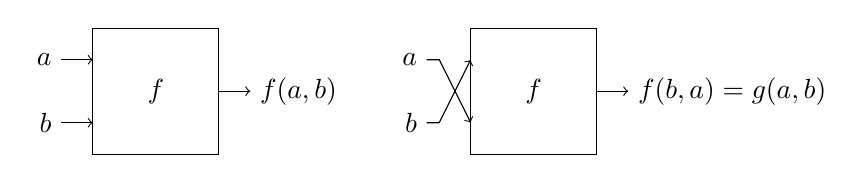
\begin{tikzpicture}[scale=0.8] %%Replaced figure with tikz figure - TWJ 6/28/2010

\draw (1,0) rectangle (3,2);
\node at (2,1)  {$f$};
\draw [->] (3,1) -- (3.5,1) node [right] {$f(a,b)$};
\draw [->] (0.5,1.5) node [left] {$a$} -- (1,1.5);
\draw [->] (0.5,0.5) node [left] {$b$} -- (1,0.5);

\draw (7,0) rectangle (9,2);
\node at (8,1)  {$f$};
\draw [->] (9,1) -- (9.5,1) node [right] {$f(b,a) = g(a,b)$};
\draw [->] (6.3,1.5) node [left] {$a$} -- (6.5,1.5) -- (7,0.5);
\draw [->] (6.3,0.5) node [left] {$b$} -- (6.5,0.5) -- (7,1.5);

\end{tikzpicture}
\end{center}

\caption{A switching function of two variables}
\label{twovar}
\end{figure}
 
 
We define a {\bfi
switching\/}\index{Function!switching}\index{Switching function} or
{\bfi Boolean
function\/}\index{Boolean function}\index{Function!Boolean} of $n$
variables to be a function from ${\mathbb Z}_2^n$ to ${\mathbb Z}_2$. Since 
any switching function can have two possible values for each binary
$n$-tuple and there are $2^n$ binary $n$-tuples, $2^{2^n}$ switching
functions are possible for $n$ variables. In general, allowing
permutations of the inputs greatly reduces the number of different
kinds of modules that are needed to build a large circuit.
 
 
The possible switching functions  with two input variables $a$ and
$b$ are listed in Table~\ref{switching_2variable}. Two switching functions $f$ and $g$
are equivalent if $g$ can be obtained from $f$ by a permutation of the
input variables. For example, $g(a, b, c) = f(b, c, a)$. In this 
case $g \sim f$ via the permutation $(acb)$. In the case of switching
functions of two variables, the permutation $(ab)$ reduces 16
possible switching functions to 12 equivalent functions since
\begin{align*}
f_2 & \sim  f_4 \\
f_3 & \sim  f_5 \\
f_{10} & \sim  f_{12} \\
f_{11} & \sim  f_{13}.
\end{align*}
 
 
\begin{table}[htb]
\caption{Switching functions in two variables}{\small
\medskip
\begin{center}
\begin{tabular}{|cc|cccccccc|}
\hline
\multicolumn{2}{|c|}{Inputs}
 & \multicolumn{8}{|c|}{Outputs}    \\
\hline
         &     & $f_0$ & $f_1$ & $f_2$ & $f_3$ & $f_4$ &
$f_5$ & $f_6$ & $f_7$  \\ \hline
0 & 0   & 0 & 0 & 0 & 0 & 0 & 0 & 0 & 0 \\
0 & 1   & 0 & 0 & 0 & 0 & 1 & 1 & 1 & 1 \\
1 & 0   & 0 & 0 & 1 & 1 & 0 & 0 & 1 & 1 \\
1 & 1   & 0 & 1 & 0 & 1 & 0 & 1 & 0 & 1 \\ \hline\hline
\multicolumn{2}{|c|}{Inputs}
 & \multicolumn{8}{|c|}{Outputs}    \\
\hline
         &     & $f_8$ & $f_9$ & $f_{10}$ & $f_{11}$
& $f_{12}$ & $f_{13}$ & $f_{14}$ & $f_{15}$ \\ \hline
0 & 0   & 1 & 1 & 1 & 1 & 1 & 1 & 1 & 1 \\
0 & 1   & 0 & 0 & 0 & 0 & 1 & 1 & 1 & 1 \\
1 & 0   & 0 & 0 & 1 & 1 & 0 & 0 & 1 & 1 \\
1 & 1   & 0 & 1 & 0 & 1 & 0 & 1 & 0 & 1 \\ \hline
\end{tabular}
\end{center}\label{switching_2variable}
}
\end{table}
 
 
For three input variables there are $2^{2^3}=256$ possible switching
functions; in the case of four variables there are $2^{2^4} =
\mbox{65,536}$. The number of equivalence classes is too large to reasonably
calculate directly. It is necessary to employ  Burnside's Theorem.
 
 
Consider a  switching function with three possible inputs, $a$, $b$,
and $c$. As we have mentioned, two switching functions $f$ and $g$ are
equivalent if a permutation of the input variables of $f$ gives $g$.
It is important to notice that a permutation of the switching
functions is not simply a permutation of the input values $\{a, b,
c\}$. A switching function is a set of output values for the inputs
$a$, $b$, and $c$, so when we consider equivalent switching functions, we
are permuting $2^3$ possible outputs, not just three input values. For
example, each binary triple $(a, b, c)$ has a specific output
associated with it. The  permutation $(acb)$ changes outputs as follows: 
\begin{align*}
(0, 0, 0) & \mapsto  (0, 0, 0) \\
(0, 0, 1) & \mapsto  (0, 1, 0) \\
(0, 1, 0) & \mapsto  (1, 0, 0) \\
& \vdots  \\
(1, 1, 0) & \mapsto  (1, 0, 1) \\
(1, 1, 1) & \mapsto  (1, 1, 1).
\end{align*}

Let $X$ be the set of output values for a switching function in $n$
variables. Then $|X|=2^n$. We can enumerate these values as follows: 
\begin{align*}
(0, \ldots, 0, 1) & \mapsto  0 \\
(0, \ldots, 1, 0) & \mapsto  1 \\
(0, \ldots, 1, 1) & \mapsto  2 \\
& \vdots  \\
(1, \ldots, 1, 1) & \mapsto  2^n-1.
\end{align*}
Now let us consider a circuit with four input variables and a single
output. Suppose that we can permute the leads  of any circuit
according to the following permutation group: 
\begin{gather*}
(a)    \quad (ac)     \quad (bd)     \quad (adcb) \\
(abcd) \quad (ab)(cd) \quad (ad)(bc) \quad (ac)(bd).
\end{gather*}
The permutations of the four possible input variables induce the
permutations of the output values in Table~\ref{switching_permute}. 
 
 

 
 
Hence, there are
\[
\frac{1}{8} (2^{16} + 2 \cdot 2^{12} + 2 \cdot 2^6 + 3 \cdot
2^{10}) = 9616
\]
possible switching functions of four variables under this group of
permutations. This number will be even smaller if we consider the full
symmetric group on four letters. 
 
 
 \begin{table}[htb]
\caption{Permutations of switching functions in four variables}{\small 
\medskip
\begin{center}
\begin{tabular}{|l|l|l|}
\hline
Group       &                                 &  Number  \\
Permutation &  Switching Function Permutation &  of Cycles  \\
\hline
$(a)$        & $(0)$ & 16 \\
$(a c)$      & $(2,8)(3,9)(6,12)(7,13)$ & 12 \\
$(b d)$      & $(1,4)(3,6)(9,12)(11,14)$ & 12 \\
$(a d c b)$  & $(1,2,4,8)(3,6.12,9)(5,10)(7,14,13,11)$ & 6\\
$(a b c d)$  & $(1,8,4,2)(3,9,12,6)(5,10)(7,11,13,14)$ & 6\\
$(a b)(c d)$ & $(1,2)(4,8)(5,10)(6,9)(7,11)(13,14)$ & 10\\
$(a d)(b c)$ & $(1,8)(2,4)(3,12)(5,10)(7,14)(11,13)$ & 10\\
$(a c)(b d)$ & $(1,4)(2,8)(3,12)(6,9)(7,13)(11,14)$ & 10 \\
\hline
\end{tabular}
\end{center}\label{switching_permute}
}
\end{table}
\histhead
 
 
 
\noindent{\small \histf
William Burnside\index{Burnside, William} was born in London in 1852.
He attended Cambridge University from 1871 to 1875 and won the Smith's
Prize in his last year.  After his graduation he lectured at
Cambridge.  He was made a member of the Royal Society in 1893.
Burnside wrote approximately 150 papers on topics in applied
mathematics, differential geometry, and probability, but his most
famous contributions were in group theory.  Several of Burnside's
conjectures have stimulated research to this day.  One such conjecture
was that every group of odd order is solvable; that is, for a group
$G$ of odd order, there exists a sequence of subgroups 
\[
G = H_n \supset H_{n-1} \supset \cdots \supset H_1 \supset
H_0 = \{ e \}
\]
such that $H_i$ is normal in $H_{i+1}$ and $H_{i+1} / H_i$ is abelian.
This conjecture was finally proven by W. Feit\index{Feit, W.}
and J. Thompson\index{Thompson, J.} in 1963. 
Burnside's  {\small \it The Theory of Groups of Finite Order},
published in 1897, was one of the first books to treat groups in a
modern context as 
opposed to permutation groups. The second edition, published in 1911,
is still a classic. 
\histbox
}
 
 
 
\markright{EXERCISES}
\section*{Exercises}
\exrule
 
 
 
 
{\small
\begin{enumerate}
 
%***************Calculations************************

% 2010/05/10 R Beezer: made it clearer what the G-equivalence classes are
\item
Examples~\ref{example:actions:GL2_action}--\ref{example:actions:left_coset_action}  in the first section each describe an action of a group $G$ on a set $X$, which will give rise to the equivalence relation defined by $G$-equivalence.  For each example, compute the equivalence classes of the equivalence relation,  the {\bfi $G$-equivalence classes\/}\index{$G$-equivalence classes}.
 
 
\item \label{actions:computation:exercise}
Compute all $X_g$ and all $G_x$ for each of the following permutation
groups. 
\begin{enumerate}
 
 \item
$X= \{1, 2, 3\}$, \\
$G=S_3=\{(1), (12), (13), (23), (123), (132)  \}$
 
 \item
$X = \{1, 2, 3, 4, 5, 6\}$, \\
$G = \{(1), (12), (345), (354), (12)(345), (12)(354)  \}$
 
\end{enumerate}
 
 
\item
Compute the $G$-equivalence classes of $X$ for each of the $G$-sets in
Exercise~\ref{actions:computation:exercise}. For each $x \in X$ verify that $|G|=|{\mathcal O}_x| \cdot
|G_x|$.  
 
 
\item
Let $G$ be the additive group of real numbers. Let the action of
$\theta \in G$ on the real plane ${\mathbb R}^2$ be given by rotating the
plane counterclockwise about the origin through $\theta$ radians. Let
$P$ be a point on the plane other than the origin.
\begin{enumerate}
 
 \item
Show that ${\mathbb R}^2$ is a $G$-set.
 
 \item
Describe geometrically the orbit containing $P$.
 
 \item
Find the group $G_P$.
 
\end{enumerate}
 
 
\item
Let $G =  A_4$ and suppose that $G$ acts on itself by conjugation;
that is, $(g,h)~\mapsto~ghg^{-1}$. 
\begin{enumerate}
 
 \item
Determine the conjugacy classes (orbits) of each element of $G$.
 
 \item
Determine all of the isotropy subgroups for each element of $G$.
 
\end{enumerate}
 
 
\item
Find the conjugacy classes and the class equation for each of the
following groups. 
\begin{multicols}{2}
\begin{enumerate}

\item
$S_4$

\item
$D_5$

\item
${\mathbb Z}_9$

\item
$Q_8$


\end{enumerate}
\end{multicols}
 

 
 
\item  %%%%%%%%%%%%%%%%
Write the class equation for $S_5$ and for $A_5$.
 
 
\item
If a square remains fixed in the plane, how many different ways can
the corners of the square be colored if three colors are used?
 
 
\item
How many ways can the vertices of an equilateral triangle be colored
using three different colors? 
 
 
\item
Find the number of ways a six-sided die can be constructed if each
side is  marked differently with $1, \ldots, 6$ 
dots.
 
\item
Up to a rotation, how many ways can the faces of a cube be colored
with three different colors? 
 
 
 
\item
Consider 12 straight wires of equal lengths with their ends soldered
together to form the edges of a cube. Either silver or copper wire can be
used for each edge.  How many different ways can the cube be
constructed? 
 
 
 
\item
Suppose that we color each of the eight corners of a cube. Using three
different colors, how many ways can the corners be colored up to a
rotation of the cube? 
 
 
\item
Each of the faces of a regular tetrahedron can be painted either red
or white.  Up to a rotation, how many different ways can the
tetrahedron be painted? 
 
 
\item
Suppose that the vertices of a regular hexagon are to be colored either
red or white.  How many ways can this be done up to a symmetry  of the
hexagon? 
 
 
\item
A molecule of benzene is made up of six carbon atoms and six hydrogen
atoms, linked together in a hexagonal shape as in Figure~\ref{benzene}.
\begin{enumerate}
 
 \item
How many different compounds can be formed by replacing one or more of
the hydrogen atoms with a chlorine atom? 
 
 \item
Find the number of different chemical compounds that can be formed by
replacing three of the six hydrogen atoms in a benzene ring with a
$CH_3$ radical.
 
\end{enumerate}
 
 
\begin{figure}[ht]
\begin{center}
\tikzpreface{actions_benzene}
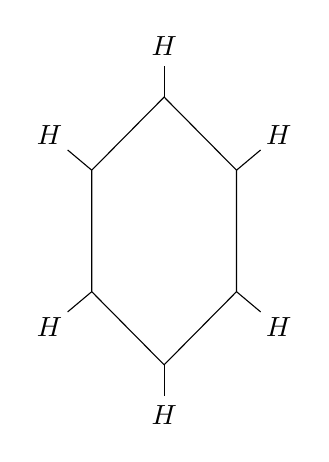
\begin{tikzpicture}[scale=1.0] %%Replaced figure with tikz figure - TWJ 6/28/2010

\draw (40:1.2) -- (90:1.7) -- (140:1.2) -- (220:1.2) -- (270:1.7) -- (320:1.2) -- cycle;
\draw (90:1.7) -- (90:2.1) node [above] {$H$};
\draw (270:1.7) -- (270:2.1) node [below] {$H$};
\draw (40:1.2) -- (40:1.6);
\node at (40:1.9) {$H$};
\draw (140:1.2) -- (140:1.6);
\node at (140:1.9) {$H$};
\draw (220:1.2) -- (220:1.6);
\node at (220:1.9) {$H$};
\draw (320:1.2) -- (320:1.6);
\node at (320:1.9) {$H$};

\end{tikzpicture}
\end{center}
\caption{A benzene ring}
\label{benzene}
\end{figure}
 
 
\item
How many equivalence classes of switching functions are there if the
input variables $x_1$, $x_2$, and $x_3$ can be permuted by any
permutation in $S_3$? What if the input variables $x_1$, $x_2$, $x_3$,
and $x_4$ can be permuted by any permutation in $S_4$?
 
 
\item
How many equivalence classes of switching functions are there if the
input variables $x_1$, $x_2$, $x_3$, and $x_4$ can be permuted by any
permutation in the subgroup of $S_4$ generated by the permutation
$(x_1 x_2 x_3 x_4)$?  
 
 
\item
A striped necktie has 12 bands of color. Each band can be colored
by one of four possible colors.  How many possible different-colored
neckties are there? 
 
 
%***************Theory******************************
 
 
\item
A group acts {\bfi faithfully\/} on a $G$-set $X$ if the identity is the
only element of $G$ that leaves every element of $X$ fixed. Show that
$G$ acts faithfully  on $X$ if and only if no two distinct elements of
$G$ have the same action on each element of $X$.
 
 
\item
Let $p$ be prime. Show that the number of different abelian groups of
order $p^n$ (up to isomorphism)  is the same as the number of
conjugacy classes in $S_n$. 
 
 
\item
Let $a \in G$. Show that for any $g \in G$, $gC(a) g^{-1} =
C(gag^{-1})$. 
 
 
\item
Let $|G| = p^n$ and suppose that $|Z(G)| = p^{n-1}$ for  $p$ prime.
Prove that $G$ is abelian. 
 
 
\item
Let $G$ be a group with order $p^n$ where $p$ is prime and $X$ a
finite $G$-set.  If $X_G = \{ x \in X : gx = x \text{ for all }g \in
G \}$ is the set of elements in $X$ fixed by the group action, then
prove that $|X| \equiv |X_G| \pmod{ p}$.

\item
If $G$ is a group of order $p^n$, where $p$ is prime and $n \geq 2$, show that $G$ must have a proper subgroup of order $p$.  If $n \geq 3$, is it true that $G$ will have a proper subgroup of order $p^2$?
%Moved problem from cosets.tex TWJ 12/19/2011
 
 
\end{enumerate}
}
 
 
 
\subsection*{Programming Exercise}
 
 
 
{\small
Write a program to compute the number of conjugacy classes in $S_n$.
What is the largest $n$ for which your program will work?
}
 
 
 
\subsection*{References and Suggested Reading} %%TWJ 6/28/2010 - References checked.
 
 
 
{\small
\begin{itemize}
 
\item[{\bf [1]}]
De Bruijin, N. G. ``P\'{o}lya's Theory of Counting,'' in {\it
Applied Combinatorial Mathematics}, Beckenbach, E. F., ed.
Wiley, New York, 1964.
 
\item[{\bf [2]}]
Eidswick, J. A. ``Cubelike Puzzles---What Are They and How
Do You Solve Them?'' {\it American Mathematical
Monthly} {\bf 93} (1986), 157--76.
 
\item[{\bf [3]}]
Harary, F., Palmer, E. M., and Robinson, R. W. ``P\'{o}lya's
Contributions to Chemical Enumeration,'' in {\it Chemical
Applications of Graph Theory}, Balaban, A. T., ed. Academic
Press, London, 1976.
 
\item[{\bf [4]}] %%TWJ 6/28/2010 - This is out of print
G{\aa}ding, L. and Tambour, T. {\it Algebra for Computer
Science}. Springer-Verlag, New York, 1988.
 
\item[{\bf [5]}] %%TWJ 6/28/2010 - This is out of print
Laufer, H. B. {\it Discrete Mathematics and Applied Modern
Algebra}. PWS-Kent, Boston, 1984.
 
 
\item[{\bf [6]}] %%TWJ 6/28/2010 - This is out of print
P\'{o}lya, G. and Read, R. C. {\it Combinatorial Enumeration
of Groups, Graphs, and Chemical Compounds}. Springer-Verlag,
New York, 1985.
 
\item[{\bf [7]}]
Shapiro, L. W. ``Finite Groups Acting on Sets with
Applications,'' {\it Mathematics Magazine}, May--June 1973,
136--47.
 
\end{itemize}
}
 
\sagesection
 
